\begin{figure}[htp]
\centering
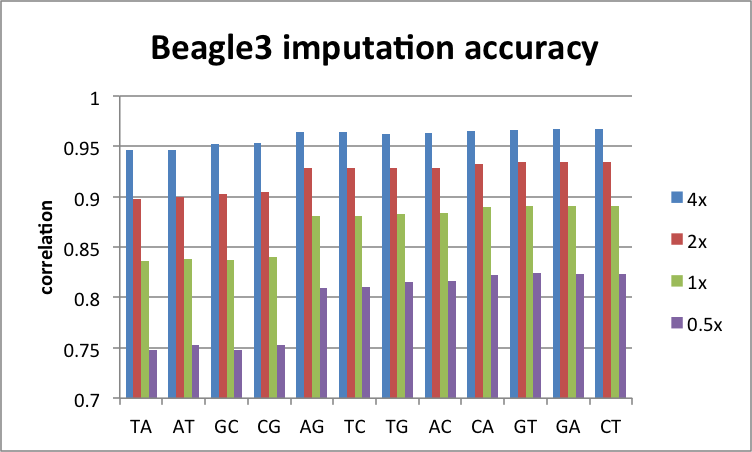
\includegraphics{Chapter3/fig/imp_accu_allele}
\caption{Imputation accuracy for each heterzygous allele. We used the Baganda 4x sequence data and SNP array data to calculate the genotype correlation for each heterozygous allele type. We found that the "mirror" alleles AT/TA and CG/GC for which it can be difficult to determine the relative strand have lower genotype correlations. }
\label{fig:imp_accu_allele}
\end{figure}